\chapter{Resultados e Discussão}
\phantom{0}
\label{sec:resultadosDisc}

Nesta seção são apresentados e detalhados os resultados dos experimentos realizados para validação do método proposto. Destaca-se que o propósito dos experimentos é investigar a aplicabilidade dos descritores de textura e os classificadores explorados nesta dissertação. Em outras palavras, o objetivo é identificar o conjunto de características que mais contribua para a classificação das categorias da camada lipídica do filme lacrimal. Além disso, é realizada uma discussão a respeito dos resultados obtidos, e uma análise comparativa (Seção~\ref{sec:comparacao}) com os trabalhos relacionados (Seção~\ref{sec:trabRelacionados}).

Os resultados estão organizados de acordo com a técnica utilizada. Na função K de \textit{Ripley} as ROIs são analisadas nos espaços de cores baseados em cores oponentes (CO), YCbCr, RGB e L*a*b*, e nos índices de diversidade filogenética em escala de cinza. Os valores apresentados representam a média das 5 repetições na validação cruzada (\textit{k-fold} = 10). São apresentadas as médias de acurácia (AC), desvio padrão em relação a acurácia (DP), \textit{Kappa}, \textit{F-Measure} (FM) e a curva ROC, destacando-se o melhor resultado em cada experimento.


\section{Experimentos utilizando a Função K de \textit{Ripley}} 
\label{sec:expKRipley}

Esta seção apresenta e discute os resultados obtidos aplicando as abordagens em círculos e anéis apresentadas sobre a função K de \textit{Ripley}. Essa técnica é realizada nas imagens das bases capturadas com o Tearscope Plus e o Interferômetro Doane.

Conforme descrito na Seção~\ref{sec:kripley}, as abordagens em círculos e anéis usando a função K de \textit{Ripley} geram 3024 características (6 raios e 6 quantizações, sendo a quantidade de variáveis de cada raio igual a 504 (254 + 128 + 64 + 32 + 16 + 8)) para cada um dos três canais de um espaço de cor, totalizando um conjunto de 9072 características. Devido à grande quantidade de variáveis extraídas, o algoritmo de seleção \textit{Greedy Stepwise} foi utilizado para reduzir a dimensionalidade, e aumentar a eficiência dos classificadores. Ciente disso, a seguir são apresentados os resultados produzidos para cada base de imagens utilizada.

\subsection{Resultados sobre as Imagens das Bases Capturadas com o Tearscope Plus}

As subseções seguintes são dedicadas para apresentar os resultados obtidos aplicando a função K de \textit{Ripley} sobre as imagens das bases VOPTICAL\_I1, VOPTICAL\_I1-v2 e VOPTICAL\_Is capturadas com o Tearscope Plus.

\subsubsection{Resultados da Base VOPTICAL\_I1}

A Tabela~\ref{tab:cirVOPTICAL_I1} apresenta a aplicação da abordagem em círculos sobre a função K de \textit{Ripley}. A maior taxa de acerto foi obtida no espaço de cor (EC) YCbCr, utilizando o classificador BN após o processo de seleção de características pelo \textit{Greedy Stepwise}, resultando em 92 variáveis selecionadas (VS). O resultado apresenta 99,23\% de acurácia, 0,79\% de desvio padrão sobre a acurácia, 0,99 de área sob a curva ROC, 0,98 de \textit{Kappa} e 0,99 de \textit{F-Measure}.

\definecolor{lightgray2}{gray}{0.8}
\begin{table}[!ht]
\centering
\onehalfspacing
\caption{Resultados produzidos sobre a base VOPTICAL\_I1, aplicando a função K de \textit{Ripley} usando abordagem em círculos.}
\label{tab:cirVOPTICAL_I1}
\resizebox{13cm}{!}{%
\begin{tabular}{llcccccc}
\cline{2-8}
 & \textbf{EC} & \multicolumn{1}{l}{\textbf{AC(\%)}} & \multicolumn{1}{l}{\textbf{DP(\%)}} & \multicolumn{1}{l}{\textbf{ROC}} & \multicolumn{1}{l}{\textbf{\textit{Kappa}}} & \multicolumn{1}{l}{\textbf{FM}} & \multicolumn{1}{l}{\textbf{VS}} \\ \cline{2-8} \parbox[t]{4mm}{\multirow{4}{*}{\rotatebox[origin=c]{90}{\textbf{BN}}}}
 & CO & 96,00 & 0,79 & 0,99 & 0,94 & 0,95 & 136 \\ 
 & \textbf{YCbCr}\cellcolor{lightgray2} & \textbf{99,23}\cellcolor{lightgray2} & \textbf{0,79}\cellcolor{lightgray2} & \textbf{0,99}\cellcolor{lightgray2} & \textbf{0,98}\cellcolor{lightgray2} & \textbf{0,99}\cellcolor{lightgray2} & \textbf{92}\cellcolor{lightgray2} \\
 & RGB & 89,52 & 0,67 & 0,98 & 0,85 & 0,89 & 90 \\
 & L*a*b* & 90,85 & 1,59 & 0,98 & 0,87 & 0,90 & 104 \\ \cline{2-8} \parbox[t]{4mm}{\multirow{4}{*}{\rotatebox[origin=c]{90}{\textbf{NB}}}}
 & CO & 96,02 & 0,79 & 0,99 & 0,94 & 0,96 & 136 \\
 & YCbCr & 99,04 & 0,67 & 0,98 & 0,98 & 0,99 & 92 \\
 & RGB & 89,14 & 1,44 & 0,98 & 0,85 & 0,89 & 90 \\
 & L*a*b* & 90,28 & 1,83 & 0,98 & 0,86 & 0,90 & 104 \\ \cline{2-8} \parbox[t]{4mm}{\multirow{4}{*}{\rotatebox[origin=c]{90}{\textbf{SVM}}}}
 & CO & 89,52 & 2,02 & 0,92 & 0,85 & 0,89 & 136 \\
 & YCbCr & 94,09 & 2,55 & 0,96 & 0,92 & 0,94 & 92 \\
 & RGB & 89,90 & 1,08 & 0,93 & 0,86 & 0,89 & 90 \\
 & L*a*b* & 88,57 & 0,95 & 0,92 & 0,84 & 0,88 & 104 \\ \cline{2-8} \parbox[t]{4mm}{\multirow{4}{*}{\rotatebox[origin=c]{90}{\textbf{RF}}}}
 & CO & 90,66 & 1,04 & 0,98 & 0,87 & 0,90 & 136 \\
 & YCbCr & 91,61 & 2,17 & 0,99 & 0,88 & 0,91 & 92 \\
 & RGB & 85,71 & 1,16 & 0,96 & 0,80 & 0,85 & 90 \\
 & L*a*b* & 87,04 & 1,27 & 0,98 & 0,82 & 0,86 & 104 \\ \cline{2-8} 
\end{tabular}
}
\end{table}

Nos testes da abordagem em anéis (Tabela~\ref{tab:aneisVOPTICAL_I1}), após o processo de seleção de características, 130 variáveis foram selecionadas no melhor caso. É possível verificar que o melhor resultado foi no espaço de cor baseado em cores oponentes e o classificador NB, apresentando 94,28\% de acurácia, 0,67\% de desvio padrão, área sob a curva ROC de 0,99, \textit{Kappa} de 0,92, \textit{F-Measure} de 0,94.

\begin{table}[!ht]
\centering
\onehalfspacing
\caption{Resultados produzidos sobre a base VOPTICAL\_I1, aplicando a função K de \textit{Ripley} usando abordagem em anéis.}
\label{tab:aneisVOPTICAL_I1}
\resizebox{13cm}{!}{%
\begin{tabular}{llcccccc}
\cline{2-8}
 & \textbf{EC} & \textbf{AC(\%)} & \textbf{DP(\%)} & \textbf{ROC} & \textbf{\textit{Kappa}} & \textbf{FM} & \textbf{VS} \\ \cline{2-8} \parbox[t]{4mm}{\multirow{4}{*}{\rotatebox[origin=c]{90}{\textbf{BN}}}}
 & CO & 93,71 & 1,44 & 0,99 & 0,91 & 0,93 & 130 \\
 & YCbCr & 93,33 & 1,16 & 0,99 & 0,91 & 0,93 & 125 \\
 & RGB & 93,71 & 1,97 & 0,99 & 0,91 & 0,93 & 104 \\
 & L*a*b* & 91,04 & 2,08 & 0,98 & 0,88 & 0,90 & 100 \\ \cline{2-8} \parbox[t]{4mm}{\multirow{4}{*}{\rotatebox[origin=c]{90}{\textbf{NB}}}}
 & \textbf{CO} \cellcolor{lightgray2} & \textbf{94,28} \cellcolor{lightgray2} & \textbf{0,67} \cellcolor{lightgray2} & \textbf{0,99} \cellcolor{lightgray2} & \textbf{0,92} \cellcolor{lightgray2} & \textbf{0,94} \cellcolor{lightgray2} & \textbf{130} \cellcolor{lightgray2} \\
 & YCbCr & 92,95 & 1,27 & 0,99 & 0,90 & 0,92 & 125 \\
 & RGB & 93,71 & 1,97 & 0,99 & 0,91 & 0,93 & 104 \\
 & L*a*b* & 90,66 & 1,83 & 0,98 & 0,87 & 0,90 & 100 \\ \cline{2-8} \parbox[t]{4mm}{\multirow{4}{*}{\rotatebox[origin=c]{90}{\textbf{SVM}}}}
 & CO & 91,42 & 2,85 & 0,94 & 0,88 & 0,91 & 130 \\
 & YCbCr & 90,09 & 2,19 & 0,93 & 0,86 & 0,90 & 125 \\
 & RGB & 89,33 & 1,24 & 0,92 & 0,85 & 0,89 & 104 \\
 & L*a*b* & 90,09 & 1,44 & 0,93 & 0,86 & 0,89 & 100 \\ \cline{2-8} \parbox[t]{4mm}{\multirow{4}{*}{\rotatebox[origin=c]{90}{\textbf{RF}}}}
 & CO & 91,61 & 1,24 & 0,98 & 0,88 & 0,91 & 130 \\
 & YCbCr & 91,23 & 1,04 & 0,98 & 0,88 & 0,91 & 125 \\
 & RGB & 90,66 & 0,79 & 0,97 & 0,87 & 0,90 & 104 \\
 & L*a*b* & 87,23 & 1,08 & 0,97 & 0,82 & 0,86 & 100 \\ \cline{2-8} 
\end{tabular}
}
\end{table}

No geral, os experimentos usando a abordagem em círculos obteve os melhores resultados para a base VOPTICAL\_I1. Apesar desse fato, pode-se notar que ambas abordagens obtiveram desempenhos promissores, apresentando na maioria dos casos resultados superiores a 90\% de acurácia, além de bons resultados nas demais métricas utilizadas.

\subsubsection{Resultados da Base VOPTICAL\_I1-v2}

A Tabela~\ref{tab:cirVOPTICAL_I1-v2} apresenta os resultados da abordagem em círculos. Após a seleção das variáveis mais relevantes, o conjunto de características foi reduzido a 84 características no melhor caso. A partir desse novo conjunto, foi obtido como melhor resultado 91,87\% de acurácia, 1,18\% de desvio padrão, 0,99 de área sob a curva ROC, 0,89 de \textit{Kappa} e 0,91 de \textit{F-Measure} sobre o espaço de cor YCbCr e usando o classificador BN.

\begin{table}[!ht]
\centering
\onehalfspacing
\caption{Resultados produzidos sobre a base VOPTICAL\_I1-v2, aplicando a função K de \textit{Ripley} usando abordagem em círculos.}
\label{tab:cirVOPTICAL_I1-v2}
\resizebox{13cm}{!}{%
\begin{tabular}{llcccccc}
\cline{2-8}
 & \textbf{EC} & \textbf{AC(\%)} & \textbf{DP(\%)} & \textbf{ROC} & \textbf{\textit{Kappa}} & \textbf{FM} & \textbf{VS} \\ \cline{2-8} \parbox[t]{4mm}{\multirow{4}{*}{\rotatebox[origin=c]{90}{\textbf{BN}}}}
 & CO & 89,68 & 0,65 & 0,98 & 0,87 & 0,89 & 114 \\
 & \textbf{YCbCr} \cellcolor{lightgray2} & \textbf{91,87} \cellcolor{lightgray2} & \textbf{1,18} \cellcolor{lightgray2} & \textbf{0,99} \cellcolor{lightgray2} & \textbf{0,89} \cellcolor{lightgray2} & \textbf{0,91} \cellcolor{lightgray2} & \textbf{84} \cellcolor{lightgray2} \\
 & RGB & 89,21 & 1,15 & 0,98 & 0,86 & 0,89 & 79 \\
 & L*a*b* & 86,87 & 2,23 & 0,98 & 0,83 & 0,86 & 119 \\ \cline{2-8} \parbox[t]{4mm}{\multirow{4}{*}{\rotatebox[origin=c]{90}{\textbf{NB}}}}
 & CO & 90,00 & 0,65 & 0,98 & 0,87 & 0,89 & 114 \\
 & YCbCr & 91,56 & 0,65 & 0,99 & 0,89 & 0,91 & 84 \\
 & RGB & 88,75 & 1,30 & 0,98 & 0,85 & 0,88 & 79 \\
 & L*a*b* & 86,56 & 1,50 & 0,98 & 0,83 & 0,86 & 119 \\ \cline{2-8} \parbox[t]{4mm}{\multirow{4}{*}{\rotatebox[origin=c]{90}{\textbf{SVM}}}}
 & CO & 86,40 & 1,18 & 0,91 & 0,82 & 0,86 & 114 \\
 & YCbCr & 84,68 & 1,18 & 0,90 & 0,80 & 0,84 & 84 \\
 & RGB & 86,56 & 1,69 & 0,91 & 0,83 & 0,86 & 79 \\
 & L*a*b* & 87,50 & 1,83 & 0,92 & 0,84 & 0,87 & 119 \\ \cline{2-8} \parbox[t]{4mm}{\multirow{4}{*}{\rotatebox[origin=c]{90}{\textbf{RF}}}}
 & CO & 86,71 & 0,95 & 0,98 & 0,83 & 0,86 & 114 \\
 & YCbCr & 90,93 & 1,41 & 0,98 & 0,88 & 0,90 & 84 \\
 & RGB & 85,15 & 1,10 & 0,97 & 0,81 & 0,85 & 79 \\
 & L*a*b* & 85,31 & 1,28 & 0,97 & 0,81 & 0,84 & 119 \\ \cline{2-8} 
\end{tabular}
}
\end{table}

A segunda abordagem (Tabela~\ref{tab:aneisVOPTICAL_I1-v2}) apresentou no melhor caso o experimento aplicando também o espaço de cor YCbCr e o classificador BN. Foi atingido uma acurácia de 93,12\%, 0,34\% de desvio padrão, 0,99 de área sob a curva ROC, 0,91 de \textit{Kappa} e 0,93 de \textit{F-Measure} sobre 89 variáveis selecionadas.

\begin{table}[!ht]
\centering
\onehalfspacing
\caption{Resultados produzidos sobre a base VOPTICAL\_I1-v2, aplicando a função K de \textit{Ripley} usando abordagem em anéis.}
\label{tab:aneisVOPTICAL_I1-v2}
\resizebox{13cm}{!}{%
\begin{tabular}{llcccccc}
\cline{2-8}
 & \textbf{EC} & \textbf{AC(\%)} & \textbf{DP(\%)} & \textbf{ROC} & \textbf{\textit{Kappa}} & \textbf{FM} & \textbf{VS} \\ \cline{2-8} \parbox[t]{4mm}{\multirow{4}{*}{\rotatebox[origin=c]{90}{\textbf{BN}}}}
 & CO & 90,93 & 1,62 & 0,99 & 0,88 & 0,90 & 102 \\
 & \textbf{YCbCr} \cellcolor{lightgray2} & \textbf{93,12} \cellcolor{lightgray2} & \textbf{0,34} \cellcolor{lightgray2} & \textbf{0,99} \cellcolor{lightgray2} & \textbf{0,91} \cellcolor{lightgray2} & \textbf{0,93} \cellcolor{lightgray2} & \textbf{89} \cellcolor{lightgray2} \\
 & RGB & 91,40 & 0,78 & 0,98 & 0,89 & 0,91 & 97 \\
 & L*a*b* & 89,53 & 1,52 & 0,98 & 0,86 & 0,89 & 103 \\ \cline{2-8} \parbox[t]{4mm}{\multirow{4}{*}{\rotatebox[origin=c]{90}{\textbf{NB}}}}
 & CO & 90,93 & 1,96 & 0,98 & 0,88 & 0,90 & 102 \\
 & YCbCr & 93,12 & 0,34 & 0,99 & 0,90 & 0,93 & 89 \\
 & RGB & 90,93 & 1,04 & 0,98 & 0,88 & 0,90 & 97 \\
 & L*a*b* & 88,75 & 1,52 & 0,98 & 0,85 & 0,88 & 103 \\ \cline{2-8} \parbox[t]{4mm}{\multirow{4}{*}{\rotatebox[origin=c]{90}{\textbf{SVM}}}}
 & CO & 90,62 & 1,23 & 0,94 & 0,88 & 0,90 & 102 \\
 & YCbCr & 87,65 & 1,69 & 0,92 & 0,84 & 0,87 & 89 \\
 & RGB & 86,87 & 1,39 & 0,91 & 0,83 & 0,86 & 97 \\
 & L*a*b* & 84,53 & 1,94 & 0,90 & 0,80 & 0,84 & 103 \\ \cline{2-8} \parbox[t]{4mm}{\multirow{4}{*}{\rotatebox[origin=c]{90}{\textbf{RF}}}}
 & CO & 91,40 & 1,99 & 0,99 & 0,89 & 0,91 & 102 \\
 & YCbCr & 90,15 & 2,44 & 0,99 & 0,87 & 0,90 & 89 \\
 & RGB & 89,06 & 0,55 & 0,97 & 0,86 & 0,88 & 97 \\
 & L*a*b* & 88,43 & 0,85 & 0,98 & 0,85 & 0,88 & 103 \\ \cline{2-8} 
\end{tabular}
}
\end{table}
\FloatBarrier

Em suma, a abordagem em anéis obteve os melhores resultados sobre a base VOPTICAL\_I1-v2. Entretanto, as duas abordagens apresentam desempenho promissor e, em ambas, os resultados aplicando o classificador BN e o espaço de cor YCbCr, superam os outros classificadores e espaços de cores. Acredita-se que, o espaço de cor YCbCr contêm informações que melhor discriminam as categorias, contribuindo com o aumento dos resultados das métricas aplicadas no classificador.

\subsubsection{Resultados da Base VOPTICAL\_Is}

Após a etapa de seleção de características para determinar as
variáveis mais relevantes, o conjunto de características foi reduzido para 120 características no melhor resultado da abordagem em círculos (Tabela~\ref{tab:cirVOPTICAL_LS}). Produziu o melhor resultado aplicando o espaço de cor YCbCr e o classificador SVM, apresentando uma acurácia de 81,52\%, desvio padrão de 0,49\%, área sob a curva ROC 0,87, \textit{Kappa} 0,73 e \textit{F-Measure} 0,81.

\begin{table}[!ht]
\centering
\onehalfspacing
\caption{Resultados produzidos sobre a base VOPTICAL\_Is, aplicando a função K de \textit{Ripley} usando abordagem em círculos.}
\label{tab:cirVOPTICAL_LS}
\resizebox{13cm}{!}{%
\begin{tabular}{llcccccc}
\cline{2-8}
 & \textbf{EC} & \textbf{AC(\%)} & \textbf{DP(\%)} & \textbf{ROC} & \textbf{\textit{Kappa}} & \textbf{FM} & \textbf{VS} \\ \cline{2-8} \parbox[t]{4mm}{\multirow{4}{*}{\rotatebox[origin=c]{90}{\textbf{BN}}}}
 & CO & 79,16 & 0,44 & 0,92 & 0,70 & 0,79 & 176 \\
 & YCbCr & 75,96 & 1,05 & 0,92 & 0,65 & 0,76 & 140 \\
 & RGB & 75,36 & 0,52 & 0,91 & 0,65 & 0,75 & 120 \\
 & L*a*b* & 75,12 & 0,93 & 0,91 & 0,64 & 0,75 & 143 \\ \cline{2-8} \parbox[t]{4mm}{\multirow{4}{*}{\rotatebox[origin=c]{90}{\textbf{NB}}}}
 & CO & 78,91 & 0,80 & 0,92 & 0,69 & 0,78 & 176 \\
 & YCbCr & 75,76 & 1,09 & 0,91 & 0,65 & 0,75 & 140 \\
 & RGB & 75,61 & 0,69 & 0,91 & 0,65 & 0,75 & 120 \\
 & L*a*b* & 74,58 & 0,63 & 0,91 & 0,63 & 0,74 & 143 \\ \cline{2-8} \parbox[t]{4mm}{\multirow{4}{*}{\rotatebox[origin=c]{90}{\textbf{SVM}}}} 
 & CO & 80,88 & 0,80 & 0,86 & 0,72 & 0,80 & 176 \\
 & \textbf{YCbCr} \cellcolor{lightgray2} & \textbf{81,52} \cellcolor{lightgray2} & \textbf{0,49} \cellcolor{lightgray2} & \textbf{0,87} \cellcolor{lightgray2} & \textbf{0,73} \cellcolor{lightgray2} & \textbf{0,81} \cellcolor{lightgray2} & \textbf{140} \cellcolor{lightgray2} \\
 & RGB & 81,28 & 0,95 & 0,86 & 0,73 & 0,81 & 120 \\
 & L*a*b* & 80,49 & 0,40 & 0,86 & 0,72 & 0,80 & 143 \\ \cline{2-8} \parbox[t]{4mm}{\multirow{4}{*}{\rotatebox[origin=c]{90}{\textbf{RF}}}}
 & CO & 78,76 & 0,70 & 0,93 & 0,68 & 0,77 & 176 \\
 & YCbCr & 78,37 & 0,58 & 0,94 & 0,68 & 0,77 & 140 \\
 & RGB & 79,16 & 0,61 & 0,93 & 0,69 & 0,78 & 120 \\
 & L*a*b* & 76,40 & 0,44 & 0,92 & 0,65 & 0,74 & 143 \\ \cline{2-8} 
\end{tabular}
}
\end{table}
\FloatBarrier

No melhor resultado da abordagem em anéis (Tabela~\ref{tab:aneisVOPTICAL_LS}), as taxas de acerto obtiveram, em média, uma melhora superior a 2 pontos em relação as taxas de acerto do melhor resultado da abordagem em círculos. Foi obtido 83,39\% de acurácia, 0,70\% de desvio padrão, 0,88 de área sob a curva ROC, 0,76 de \textit{Kappa}, 0,83 de \textit{F-Measure}, sobre 176 variáveis selecionadas do conjunto de características, no espaço de cor YCbCr, usando o classificador SVM.

\begin{table}[!ht]
\centering
\onehalfspacing
\caption{Resultados produzidos sobre a base VOPTICAL\_Is, aplicando a função K de \textit{Ripley} usando abordagem em anéis.}
\label{tab:aneisVOPTICAL_LS}
\resizebox{13cm}{!}{%
\begin{tabular}{llcccccc}
\cline{2-8}
 & \textbf{EC} & \textbf{AC(\%)} & \textbf{DP(\%)} & \textbf{ROC} & \textbf{\textit{Kappa}} & \textbf{FM} & \textbf{VS} \\ \cline{2-8} \parbox[t]{4mm}{\multirow{4}{*}{\rotatebox[origin=c]{90}{\textbf{BN}}}}
 & CO & 80,78 & 0,87 & 0,93 & 0,72 & 0,80 & 188 \\
 & YCbCr & 81,57 & 1,05 & 0,94 & 0,73 & 0,81 & 176 \\
 & RGB & 78,52 & 0,66 & 0,93 & 0,69 & 0,78 & 148 \\
 & L*a*b* & 77,98 & 1,16 & 0,94 & 0,68 & 0,78 & 169 \\ \cline{2-8} \parbox[t]{4mm}{\multirow{4}{*}{\rotatebox[origin=c]{90}{\textbf{NB}}}}
 & CO & 81,23 & 0,82 & 0,93 & 0,73 & 0,81 & 188 \\
 & YCbCr & 81,03 & 1,00 & 0,94 & 0,73 & 0,81 & 176 \\
 & RGB & 78,42 & 0,37 & 0,93 & 0,69 & 0,78 & 148 \\
 & L*a*b* & 77,93 & 1,10 & 0,93 & 0,68 & 0,78 & 169 \\ \cline{2-8} \parbox[t]{4mm}{\multirow{4}{*}{\rotatebox[origin=c]{90}{\textbf{SVM}}}}
 & CO & 82,75 & 0,87 & 0,87 & 0,75 & 0,82 & 188 \\
 & \textbf{YCbCr} \cellcolor{lightgray2} & \textbf{83,39} \cellcolor{lightgray2} & \textbf{0,70} \cellcolor{lightgray2} & \textbf{0,88} \cellcolor{lightgray2} & \textbf{0,76} \cellcolor{lightgray2} & \textbf{0,83} \cellcolor{lightgray2} & \textbf{176} \cellcolor{lightgray2} \\
 & RGB & 80,78 & 1,47 & 0,86 & 0,72 & 0,80 & 148 \\
 & L*a*b* & 78,57 & 0,17 & 0,84 & 0,69 & 0,77 & 169 \\ \cline{2-8} \parbox[t]{4mm}{\multirow{4}{*}{\rotatebox[origin=c]{90}{\textbf{RF}}}}
 & CO & 77,19 & 1,32 & 0,94 & 0,66 & 0,76 & 188 \\
 & YCbCr & 79,06 & 0,42 & 0,95 & 0,69 & 0,77 & 176 \\
 & RGB & 78,22 & 1,53 & 0,93 & 0,68 & 0,76 & 148 \\
 & L*a*b* & 77,73 & 0,66 & 0,94 & 0,67 & 0,76 & 169 \\ \cline{2-8} 
\end{tabular}
}
\end{table}

Os experimentos analisados nas abordagens em círculos e anéis sobre a base VOPTICAL\_Is, obtiveram as taxas de acerto mais baixas em comparação com os resultados das bases de imagens VOPTICAL\_I1, VOPTICAL\_I1-v2 capturadas com o Tearscope Plus. Uma das possíveis causas pode ser a produção de características não-discriminativas para o problema específico, pois como descrito na Seção~\ref{subsec:basesI1eIs} as imagens que compõe esta base apresentam iluminação irregular. Entretanto, as taxas de acerto apresentam resultados razoáveis e bastantes promissores, visto que, a base de imagens é extremamente desbalanceada, variando de 40 a 117 imagens entre as categorias, o que possivelmente seja a causa principal para os resultados obtidos.

\subsection{Resultados sobre as Imagens das Bases Capturadas com o Interferômetro Doane}

A subseção seguinte apresenta os resultados obtidos aplicando a função K de \textit{Ripley} sobre as imagens a base VOPTICAL\_GCU capturada com o Interferômetro Doane.

\subsubsection{Resultados da Base VOPTICAL\_GCU}

A Tabela~\ref{tab:cirVOPTICAL_GCU} apresenta os experimentos aplicando a abordagem em círculos. Pode ser analisado que o melhor resultado foi obtido no espaço de cor YCbCr e usando o classificador BN, após a seleção de 106 variáveis. O resultado apresenta uma acurácia de 95,28\%, desvio padrão de 0,94, área sob a curva ROC de 0,99, \textit{Kappa} de 0,93 e 0,95 de \textit{F-Measure}.

\begin{table}[!ht]
\centering
\onehalfspacing
\caption{Resultados produzidos sobre a base VOPTICAL\_GCU, aplicando a função K de \textit{Ripley} usando abordagem em círculos.}
\label{tab:cirVOPTICAL_GCU}
\resizebox{13cm}{!}{%
\begin{tabular}{llcccccc}
\cline{2-8}
 & \textbf{EC} & \textbf{AC(\%)} & \textbf{DP(\%)} & \textbf{ROC} & \textbf{\textit{Kappa}} & \textbf{FM} & \textbf{VS} \\ \cline{2-8} \parbox[t]{4mm}{\multirow{4}{*}{\rotatebox[origin=c]{90}{\textbf{BN}}}}
 & CO & 94,40 & 0,84 & 0,99 & 0,93 & 0,95 & 115 \\
 & \textbf{YCbCr} \cellcolor{lightgray2} & \textbf{95,28} \cellcolor{lightgray2} & \textbf{0,94} \cellcolor{lightgray2} & \textbf{0,99} \cellcolor{lightgray2} & \textbf{0,93} \cellcolor{lightgray2} & \textbf{0,95} \cellcolor{lightgray2} & \textbf{106} \cellcolor{lightgray2} \\
 & RGB & 91,13 & 1,43 & 0,98 & 0,88 & 0,90 & 99 \\
 & L*a*b* & 93,96 & 1,43 & 0,99 & 0,92 & 0,94 & 106 \\ \cline{2-8} \parbox[t]{4mm}{\multirow{4}{*}{\rotatebox[origin=c]{90}{\textbf{NB}}}}
 & CO & 94,15 & 0,78 & 0,99 & 0,92 & 0,94 & 115 \\
 & YCbCr & 94,71 & 1,07 & 0,99 & 0,93 & 0,94 & 106 \\
 & RGB & 90,56 & 0,94 & 0,98 & 0,88 & 0,90 & 99 \\
 & L*a*b* & 94,15 & 0,78 & 0,99 & 0,92 & 0,94 & 106 \\ \cline{2-8} \parbox[t]{4mm}{\multirow{4}{*}{\rotatebox[origin=c]{90}{\textbf{SVM}}}}
 & CO & 87,92 & 1,55 & 0,92 & 0,84 & 0,86 & 115 \\
 & YCbCr & 85,28 & 2,17 & 0,90 & 0,80 & 0,85 & 106 \\
 & RGB & 83,58 & 2,63 & 0,89 & 0,78 & 0,82 & 99 \\
 & L*a*b* & 89,05 & 1,07 & 0,92 & 0,85 & 0,88 & 106 \\ \cline{2-8} \parbox[t]{4mm}{\multirow{4}{*}{\rotatebox[origin=c]{90}{\textbf{RF}}}}
 & CO & 89,62 & 0,10 & 0,98 & 0,86 & 0,86 & 115 \\
 & YCbCr & 89,62 & 0,66 & 0,98 & 0,86 & 0,88 & 106 \\
 & RGB & 85,84 & 1,76 & 0,97 & 0,81 & 0,84 & 99 \\
 & L*a*b* & 85,84 & 1,15 & 0,98 & 0,81 & 0,84 & 106 \\ \cline{2-8} 
\end{tabular}
}
\end{table}
\FloatBarrier

Analisando os resultados dos experimentos da abordagem em anéis apresentado na Tabela~\ref{tab:aneisVOPTICAL_GCU}, é possível verificar que o melhor resultado foi usando o espaço de cor baseado em cores oponentes e o classificador BN, sobre 129 variáveis selecionadas. Os resultados obtidos para acurácia, desvio padrão, área sob a curva ROC, \textit{Kappa} e \textit{F-Measure} são 95,09\%, 1,81\%, 0,99, 0,93 e 0,95 respectivamente.

Em geral, os experimentos realizados sobre as duas abordagens aplicadas sobre a base VOPTICAL\_GCU, demonstram que os resultados se comportam de maneira semelhante, evidenciando que as abordagens testadas representam bem o padrão de textura das amostras das categorias da camada lipídica do filme lacrimal, para a referida base.

\begin{table}[!ht]
\centering
\onehalfspacing
\caption{Resultados produzidos sobre a base VOPTICAL\_GCU, aplicando a função K de \textit{Ripley} usando abordagem em anéis.}
\label{tab:aneisVOPTICAL_GCU}
\resizebox{13cm}{!}{%
\begin{tabular}{llcccccc}
\cline{2-8} 
 & \textbf{EC} & \multicolumn{1}{r}{\textbf{AC(\%)}} & \multicolumn{1}{r}{\textbf{DP(\%)}} & \multicolumn{1}{r}{\textbf{ROC}} & \multicolumn{1}{r}{\textbf{\textit{Kappa}}} & \multicolumn{1}{r}{\textbf{FM}} & \multicolumn{1}{r}{\textbf{VS}} \\ \cline{2-8} \parbox[t]{4mm}{\multirow{4}{*}{\rotatebox[origin=c]{90}{\textbf{BN}}}} 
 & \textbf{CO} \cellcolor{lightgray2} & \textbf{95,09} \cellcolor{lightgray2} & \textbf{1,81} \cellcolor{lightgray2} & \textbf{0,99} \cellcolor{lightgray2} & \textbf{0,93} \cellcolor{lightgray2} & \textbf{0,95} \cellcolor{lightgray2} & \textbf{129} \cellcolor{lightgray2} \\
 & YCbCr & 94,52 & 1,03 & 0,99 & 0,92 & 0,94 & 146 \\
 & RGB & 92,26 & 1,03 & 0,98 & 0,90 & 0,92 & 101 \\
 & L*a*b* & 93,96 & 1,07 & 0,99 & 0,92 & 0,94 & 133 \\ \cline{2-8} \parbox[t]{4mm}{\multirow{4}{*}{\rotatebox[origin=c]{90}{\textbf{NB}}}}
 & CO & 94,90 & 1,57 & 0,99 & 0,93 & 0,94 & 129 \\
 & YCbCr & 94,33 & 1,33 & 0,99 & 0,92 & 0,94 & 146 \\
 & RGB & 91,69 & 1,23 & 0,98 & 0,89 & 0,91 & 101 \\
 & L*a*b* & 92,45 & 0,66 & 0,99 & 0,90 & 0,92 & 133 \\ \cline{2-8} \parbox[t]{4mm}{\multirow{4}{*}{\rotatebox[origin=c]{90}{\textbf{SVM}}}}
 & CO & 82,64 & 1,95 & 0,88 & 0,77 & 0,80 & 129 \\
 & YCbCr & 90,56 & 1,15 & 0,93 & 0,87 & 0,90 & 146 \\
 & RGB & 91,32 & 0,78 & 0,94 & 0,88 & 0,90 & 101 \\
 & L*a*b* & 92,07 & 1,26 & 0,94 & 0,89 & 0,92 & 133 \\ \cline{2-8} \parbox[t]{4mm}{\multirow{4}{*}{\rotatebox[origin=c]{90}{\textbf{RF}}}}
 & CO & 83,39 & 2,06 & 0,98 & 0,78 & 0,80 & 129 \\
 & YCbCr & 87,54 & 0,42 & 0,99 & 0,83 & 0,85 & 146 \\
 & RGB & 88,11 & 0,51 & 0,97 & 0,84 & 0,85 & 101 \\
 & L*a*b* & 87,73 & 1,15 & 0,98 & 0,83 & 0,86 & 133 \\ \cline{2-8} 
\end{tabular}
}
\end{table}
\FloatBarrier

\section{Experimentos utilizando os Índices de Diversidade Filogenética}
\label{sec:expKRipley}

Nesta seção são apresentados os resultados com os descritores de textura baseados em índices de diversidade filogenética, extraídos em escala de cinza. Os experimentos foram realizados para cada grupo de índices, conforme descrito na Seção~\ref{sec:indicesDiversidade}. Essa técnica foi aplicada nas imagens da base capturadas com o Interferômetro Doane.

\subsection{Resultados da Base VOPTICAL\_GCU}
\label{subsectionVOPTICAL_GCU}

A Tabela~\ref{tab:indicesFilogeneticosVOPTICAL_GCU} apresenta os resultados dos índices de diversidade filogenética baseados em caminho mínimo, distância entre pares de espécies e topologia. É possível observar que os resultados de cada grupo são promissores. No melhor caso, tem-se quando combinados todos os índices de diversidade filogenética, usando o classificador RF. Foi alcançado uma acurácia de 97,36\%, desvio padrão de 0,78\%, área sob a curva ROC de 0,99, \textit{Kappa} de 0,96 e \textit{F-Measure} de 0,97.

\begin{table}[!ht]
\centering
\onehalfspacing
\caption{Resultados produzidos sobre a base VOPTICAL\_GCU, aplicando os grupos de índices de diversidade filogenética.}
\label{tab:indicesFilogeneticosVOPTICAL_GCU}
\resizebox{13cm}{!}{%
\begin{tabular}{llccccc}
\cline{2-7}
 & \textbf{\begin{tabular}[c]{@{}l@{}}Índices baseados \\ em:\end{tabular}} & \textbf{AC(\%)} & \textbf{DP(\%)} & \textbf{ROC} & \textbf{\textit{Kappa}} & \textbf{FM} \\ \cline{2-7} \parbox[t]{4mm}{\multirow{5}{*}{\rotatebox[origin=c]{90}{\textbf{BN}}}}
 & Caminho mínimo & 97,34 & 0,42 & 0,98 & 0,96 & 0,97 \\
 & \begin{tabular}[c]{@{}l@{}}Distância entre pares\\ de espécies\end{tabular} & 94,33 & 1,15 & 0,98 & 0,92 & 0,94 \\
 & Topologia & 95,84 & 0,51 & 0,97 & 0,94 & 0,95 \\
 & Todos os índices & 94,90 & 0,51 & 0,99 & 0,93 & 0,94 \\ \cline{2-7} \parbox[t]{4mm}{\multirow{5}{*}{\rotatebox[origin=c]{90}{\textbf{NB}}}}
 & Caminho mínimo & 97,34 & 0,42 & 0,97 & 0,96 & 0,97 \\
 & \begin{tabular}[c]{@{}l@{}}Distância entre pares\\ de espécies\end{tabular} & 94,90 & 0,84 & 0,98 & 0,93 & 0,94 \\
 & Topologia & 95,84 & 0,51 & 0,97 & 0,94 & 0,95 \\
 & Todos os índices & 94,90 & 0,51 & 0,99 & 0,93 & 0,94 \\ \cline{2-7} \parbox[t]{4mm}{\multirow{5}{*}{\rotatebox[origin=c]{90}{\textbf{SVM}}}}
 & Caminho mínimo & 93,20 & 0,42 & 0,95 & 0,91 & 0,93 \\
 & \begin{tabular}[c]{@{}l@{}}Distância entre pares\\ de espécies\end{tabular} & 94,71 & 1,57 & 0,96 & 0,93 & 0,94 \\
 & Topologia & 95,66 & 0,84 & 0,94 & 0,94 & 0,95 \\
 & Todos os índices & 93,58 & 1,68 & 0,96 & 0,91 & 0,93 \\ \cline{2-7} \parbox[t]{4mm}{\multirow{5}{*}{\rotatebox[origin=c]{90}{\textbf{RF}}}}
 & Caminho mínimo & 96,79 & 0,84 & 0,99 & 0,95 & 0,96 \\
 & \begin{tabular}[c]{@{}l@{}}Distância entre pares\\ de espécies\end{tabular} & 94,71 & 1,26 & 0,99 & 0,93 & 0,94 \\
 & Topologia & 95,84 & 0,51 & 0,99 & 0,94 & 0,95 \\
 & \textbf{Todos os índices} \cellcolor{lightgray2} & \textbf{97,36} \cellcolor{lightgray2} & \textbf{0,78} \cellcolor{lightgray2} & \textbf{0,99} \cellcolor{lightgray2} & \textbf{0,96} \cellcolor{lightgray2} & \textbf{0,97} \cellcolor{lightgray2} \\ \cline{2-7} 
\end{tabular}
}
\end{table}
\FloatBarrier

É importante destacar que os índices baseados no caminho mínimo demonstraram o segundo melhor resultado, acredita-se que isso ocorre porque a informação extraída relacionada ao grau de parentesco (diversidade) entre as espécies consegue ser bem evidenciada, uma vez que esse tem seu comportamento central baseado na raiz da árvore filogenética. Além disso, os resultados são balanceados e consistentes em todos os grupos dos índices de diversidade, alcançando sempre valores acima de 93\% acurácia. Além disso, os valores de desvios padrão são baixos, apresentando, em média, valores inferiores a 2\% e a área sob a curva ROC, \textit{Kappa} e \textit{F-Measure} resultados superiores a 0,93.

\section{Experimentos utilizando os Índices de Diversidade Filogenética e a Função K de \textit{Ripley}}

Nesta seção são apresentados os resultados obtidos utilizando as duas abordagens da função K de \textit{Ripley} e os índices de diversidade filogenética, sobre as imagens da base VOPTICAL\_GCU capturadas com o Interferômetro Doane.

\subsection{Resultados da Base VOPTICAL\_GCU}

Com o objetivo de alcançar as maiores taxas de acerto, foi realizado uma grande quantidade de testes, que consistiam de experimentos de classificação com diversas combinações dos índices de diversidade filogenética e a função K de \textit{Ripley} com suas abordagens. Buscava-se encontrar o conjunto de características mais discriminativas para classificar as categorias da camada lipídica do filme lacrimal.

\begin{table}[!ht]
\centering
\onehalfspacing
\caption{Resultados produzidos sobre a base VOPTICAL\_GCU, combinando todos os grupos de índices de diversidade filogenética e a função K de \textit{Ripley} usando a abordagem em círculos.}
\label{tab:cirIndicesFKRipleyVOPTICAL_GCU}
\resizebox{13cm}{!}{%
\begin{tabular}{llcccccc}
\cline{2-8}
 & \textbf{EC} & \textbf{AC(\%)} & \textbf{DP(\%)} & \textbf{ROC} & \textbf{\textit{Kappa}} & \textbf{FM} & \textbf{VS} \\ \cline{2-8} \parbox[t]{4mm}{\multirow{4}{*}{\rotatebox[origin=c]{90}{\textbf{BN}}}}
 & CO + Cinza & 98,11 & 0,10 & 0,99 & 0,97 & 0,98 & 81 \\
 & YCbCr + Cinza & 97,73 & 0,51 & 0,99 & 0,97 & 0,97 & 88 \\
 & RGB + Cinza & 98,49 & 0,51 & 0,99 & 0,98 & 0,98 & 54 \\
 & L*a*b* + Cinza & 96,60 & 0,51 & 0,99 & 0,95 & 0,96 & 69 \\ \cline{2-8} \parbox[t]{4mm}{\multirow{4}{*}{\rotatebox[origin=c]{90}{\textbf{NB}}}}
 & CO + Cinza & 97,54 & 0,51 & 0,99 & 0,96 & 0,97 & 81 \\
 & YCbCr + Cinza & 97,54 & 0,84 & 0,99 & 0,96 & 0,97 & 88 \\
 & RGB + Cinza & 98,30 & 0,42 & 0,99 & 0,97 & 0,98 & 54 \\
 & L*a*b* + Cinza & 96,98 & 1,03 & 0,99 & 0,96 & 0,97 & 69 \\ \cline{2-8} \parbox[t]{4mm}{\multirow{4}{*}{\rotatebox[origin=c]{90}{\textbf{SVM}}}}
 & CO + Cinza & 92,83 & 1,71 & 0,95 & 0,90 & 0,92 & 81 \\
 & YCbCr + Cinza & 94,52 & 1,23 & 0,96 & 0,92 & 0,94 & 88 \\
 & RGB + Cinza & 95,09 & 0,78 & 0,96 & 0,93 & 0,95 & 54 \\
 & L*a*b* + Cinza & 97,54 & 0,84 & 0,98 & 0,96 & 0,97 & 69 \\ \cline{2-8} \parbox[t]{4mm}{\multirow{4}{*}{\rotatebox[origin=c]{90}{\textbf{RF}}}}
 & CO + Cinza & 98,11 & 0,66 & 0,99 & 0,97 & 0,98 & 81 \\
 & YCbCr + Cinza & 98,49 & 0,51 & 0,99 & 0,98 & 0,98 & 88 \\
 & \textbf{RGB + Cinza} \cellcolor{lightgray2} & \textbf{99,81} \cellcolor{lightgray2} & \textbf{0,42} \cellcolor{lightgray2} & \textbf{0,99} \cellcolor{lightgray2} & \textbf{0,99} \cellcolor{lightgray2} & \textbf{0,99} \cellcolor{lightgray2} & \textbf{54} \cellcolor{lightgray2} \\
 & L*a*b* + Cinza & 98,67 & 0,51 & 0,99 & 0,98 & 0,98 & 69 \\ \cline{2-8} 
\end{tabular}
}
\end{table}

Após a bateria de testes, o conjunto de características que produziu as maiores taxas de acerto foi com a combinação de todos os grupos dos índices de diversidade filogenética em conjunto com a função K de \textit{Ripley}. O resultado da combinação dos índices de diversidade e a função K de \textit{Ripley} usando abordagem em círculos é apresentado na Tabela~\ref{tab:cirIndicesFKRipleyVOPTICAL_GCU}. É possível observar que o melhor caso foi obtido usando o classificador RF, no espaço de cor RGB para a função K de \textit{Ripley} e em escala de cinza para os índices de diversidade, alcançando uma acurácia de 99,81\%, desvio padrão de 0,42\%, área sob a curva ROC de 0,99, \textit{Kappa} de 0,99, \textit{F-Measure} de 0,99 e foram selecionadas 54 variáveis.

\begin{table}[!ht]
\centering
\onehalfspacing
\caption{Resultados produzidos sobre a base VOPTICAL\_GCU, combinando todos os grupos de índices de diversidade filogenética e a função K de \textit{Ripley} usando a abordagem em anéis.}
\label{tab:aneisIndicesFKRipleyVOPTICAL_GCU}
\resizebox{13cm}{!}{%
\begin{tabular}{llcccccc}
\cline{2-8}
 & \textbf{EC} & \textbf{AC(\%)} & \textbf{DP(\%)} & \textbf{ROC} & \textbf{\textit{Kappa}} & \textbf{FM} & \textbf{VS} \\ \cline{2-8} \parbox[t]{4mm}{\multirow{4}{*}{\rotatebox[origin=c]{90}{\textbf{BN}}}}
 & CO + Cinza & 99,05 & 0,10 & 0,99 & 0,98 & 0,99 & 89 \\
 & YCbCr + Cinza & 97,73 & 0,51 & 0,97 & 0,97 & 0,99 & 111 \\
 & RGB + Cinza & 98,30 & 0,78 & 0,99 & 0,97 & 0,98 & 85 \\
 & L*a*b* + Cinza & 97,54 & 0,51 & 0,99 & 0,96 & 0,97 & 89 \\ \cline{2-8} \parbox[t]{4mm}{\multirow{4}{*}{\rotatebox[origin=c]{90}{\textbf{NB}}}}
 & CO + Cinza & 99,05 & 0,04 & 0,99 & 0,98 & 0,99 & 89 \\
 & YCbCr + Cinza & 97,73 & 0,516 & 0,99 & 0,97 & 0,97 & 111 \\
 & RGB + Cinza & 98,49 & 1,07 & 0,99 & 0,98 & 0,98 & 85 \\
 & L*a*b* + Cinza & 97,73 & 0,84 & 0,99 & 0,97 & 0,97 & 89 \\ \cline{2-8} \parbox[t]{4mm}{\multirow{4}{*}{\rotatebox[origin=c]{90}{\textbf{SVM}}}}
 & CO + Cinza & 94,33 & 1,49 & 0,96 & 0,92 & 0,94 & 89 \\
 & YCbCr + Cinza & 96,79 & 0,51 & 0,98 & 0,95 & 0,96 & 111 \\
 & RGB + Cinza & 93,58 & 0,78 & 0,95 & 0,91 & 0,93 & 85 \\
 & L*a*b* + Cinza & 96,22 & 0,94 & 0,97 & 0,95 & 0,96 & 89 \\ \cline{2-8} \parbox[t]{4mm}{\multirow{4}{*}{\rotatebox[origin=c]{90}{\textbf{RF}}}}
 & \textbf{CO + Cinza} \cellcolor{lightgray2} & \textbf{99,43} \cellcolor{lightgray2} & \textbf{0,51} \cellcolor{lightgray2} & \textbf{0,99} \cellcolor{lightgray2} & \textbf{0,99} \cellcolor{lightgray2} & \textbf{0,99} \cellcolor{lightgray2} & \textbf{89} \cellcolor{lightgray2} \\
 & YCbCr + Cinza & 98,49 & 0,51 & 0,99 & 0,98 & 0,98 & 111 \\
 & RGB + Cinza & 97,92 & 0,78 & 0,99 & 0,97 & 0,97 & 85 \\
 & L*a*b* + Cinza & 97,92 & 0,42 & 0,99 & 0,97 & 0,97 & 89 \\ \cline{2-8} 
\end{tabular}
}
\end{table}

A Tabela~\ref{tab:aneisIndicesFKRipleyVOPTICAL_GCU} mostra os resultados dos experimentos usando a função K de \textit{Ripley} na abordagem em anéis, e os índices de diversidade filogenética. O melhor resultado foi obtido usando o classificador RF no espaço de cor baseado em cores oponentes para a função K de \textit{Ripley} e em escala de cinza para os índices de diversidade. Do conjunto de 89 variáveis selecionadas, obteve-se uma acurácia de 99,43\% com desvio padrão de 0,51\%, área sob a curva ROC de 0,99, \textit{Kappa} de 0,99 e \textit{F-Measure} de 0,99.

Em geral, comparando os resultados apresentados nas Tabelas~\ref{tab:cirIndicesFKRipleyVOPTICAL_GCU} e~\ref{tab:aneisIndicesFKRipleyVOPTICAL_GCU}, pode-se observar que a abordagem em anéis obteve os melhores resultados. Entretanto, pode-se notar que ambas as abordagens obtiveram desempenhos satisfatórios. Portanto, ao combinar os índices de diversidade com a árvore filogenética e a função K de \textit{Ripley}, foi possível obter um ótimo fator discriminante, que resultou em uma acurácia de mais de 99\% usando o classificador RF para classificação da camada lipídica do filme lacrimal.

\section{Resumo dos Resultados}

Esta seção apresenta o resumo dos principais resultados produzidos pelos experimentos demonstrados na Seção~\ref{sec:resultadosDisc}. As Figuras~\ref{fig:graficoKRipley},~\ref{fig:graficoIndicesDF} e~\ref{fig:graficoIndicesDFKRipley} apresentam os gráficos dos resultados obtidos em termo de acurácia para os descritores abordados neste trabalho.

\begin{figure}[!ht]
    \centering
    \caption{Gráfico dos principais resultados da função K de \textit{Ripley} para todas as bases de imagens.}
    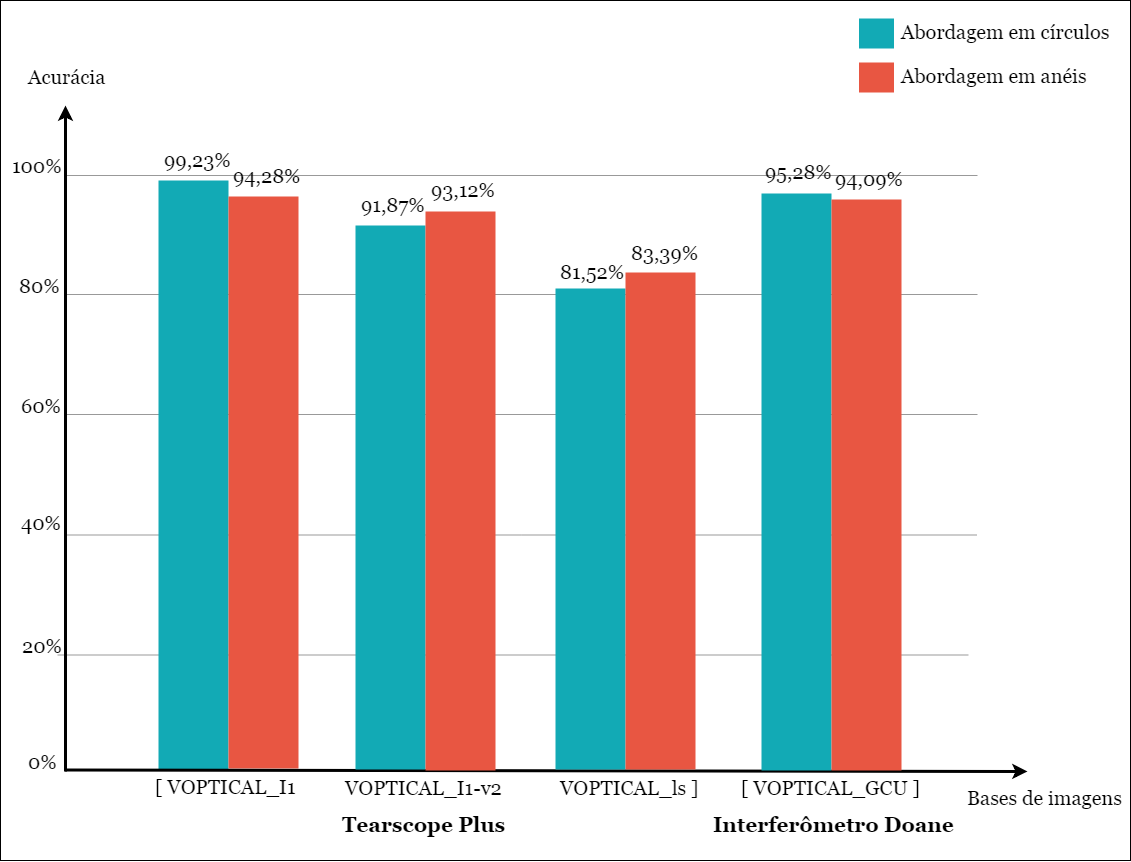
\includegraphics[width=0.8\textwidth]{figs/graficoKRipley1.png}
    \legend{Fonte: Elaborado pela autora.}
    \label{fig:graficoKRipley}
\end{figure}

A Figura~\ref{fig:graficoKRipley} ilustra o gráfico dos melhores resultados das abordagens em círculos e anéis da função K de \textit{Ripley} para todas as bases de imagens, empregada nesta dissertação. Nas bases de imagens capturadas com o Tearscope Plus os melhores resultados foram usando a abordagem em anéis, somente a base VOPTICAL\_I1 obteve melhor resultado utilizando a abordagem em círculos. Acredita-se que, as amostras adicionadas na versão atualizada (VOPTICAL\_I1-v2) apresentaram melhor comportamento com as características extraídas da abordagem em anéis, do que as amostras da primeira versão.

Por outro lado, a base de imagens VOPTICAL\_GCU capturada com o Interferômetro Doane, apresenta o melhor resultado usando a abordagem em círculos. Pressupõe-se que, para esse tipo de imagens as informações cumulativas sobre as regiões do objeto, fornecidas pelo uso de círculos são necessárias, pois as regiões centrais contém informações relevantes para a discriminação das imagens. Além disso, é importante enfatizar que ambas abordagens produziram bons resultados para os diferentes tipos de imagens utilizadas no método proposto. Dessa forma, conclui-se que as características extraídas da função K de \textit{Ripley} aplicadas sobre ambas abordagens, possuem um alto poder de discriminação dos padrões de interferência da camada lipídica do filme lacrimal.

%É importante enfatizar que um número maior de amostras aumenta a heterogeneidade e, consequentemente leva os experimentos a estarem sob circunstâncias mais realistas. Tendo em vista isto, é possível verificar que as bases de imagens VOPTICAL\_I1-v2 e VOPTICAL\_Is possuem um número maior de amostras e apresentam bons resultados, sendo bastante similares entre as abordagens. Portanto, conclui-se que as características extraídas da função K de \textit{Ripley} aplicadas sobre ambas abordagens, possuem um alto poder de discriminação dos padrões de interferência da camada lipídica do filme lacrimal.

\begin{figure}[!ht]
    \centering
    \caption{Gráfico dos principais resultados dos índices de diversidade filogenética para a base VOPTICAL\_GCU.}
    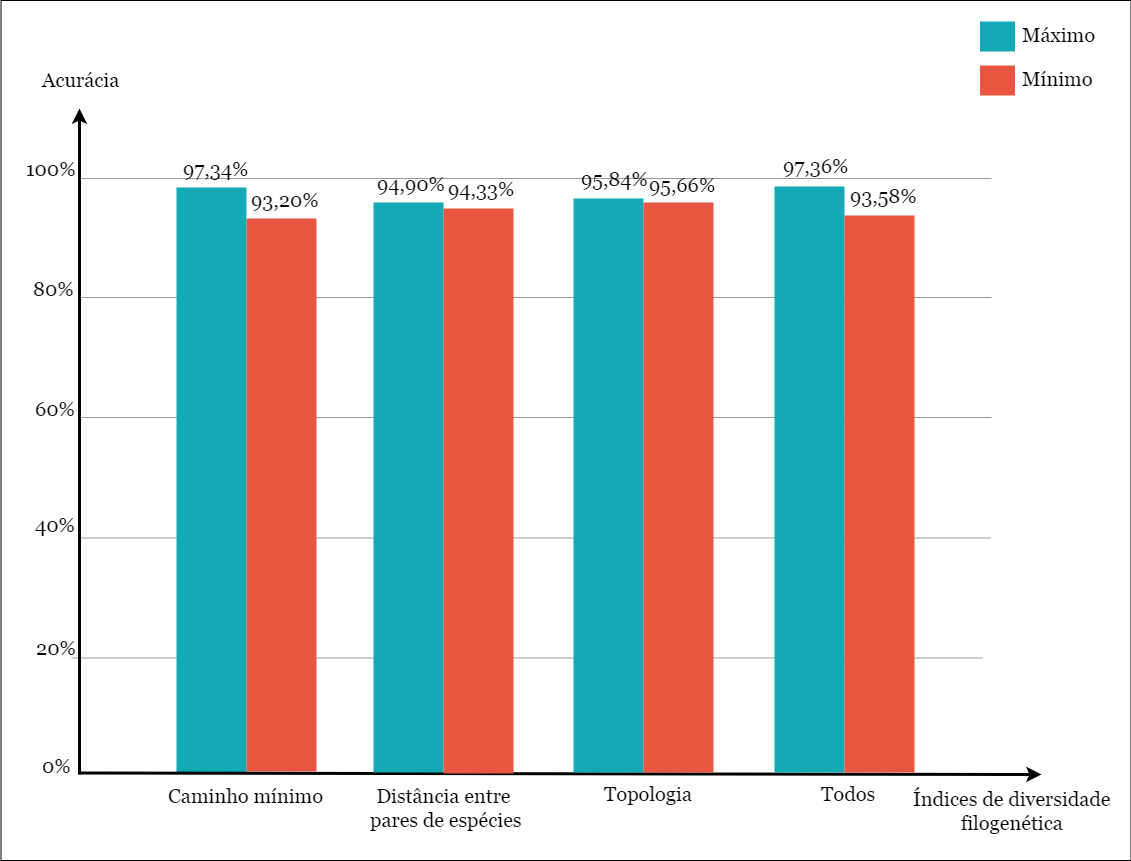
\includegraphics[width=0.8\textwidth]{figs/graficoIndices1.png}
    \legend{Fonte: Elaborado pela autora.}
    \label{fig:graficoIndicesDF}
\end{figure}

O gráfico da Figura~\ref{fig:graficoIndicesDF} apresenta o melhor e o pior resultado produzido por cada grupo dos índices de diversidade filogenética para a base de imagens VOPTICAL\_GCU capturada com o Interferômetro Doane. Ao analisar os resultados, verifica-se que o melhor desempenho foi obtido ao combinar todos os índices de diversidade filogenética. Em suma, acredita-se que a combinação de todos os índices de diversidade permite uma melhor discriminação porque os índices se complementam, isto é, um índice pode destacar uma propriedade que outro não consegue.

Em relação aos piores desempenhos, pode-se observar que a maioria foram obtidos usando o classificador SVM, conforme extraídos dos resultados apresentados na Subseção~\ref{subsectionVOPTICAL_GCU}. O SVM foi originalmente projetado para classificação binária \cite{hsu2002comparison}, e o problema proposto neste trabalho trata-se de uma abordagem multiclasse. Logo, presume-se que ao aumentar o número de classes o classificador diminui seu poder de discriminação, apresentando resultados inferiores. Entretanto, a média dos piores resultados é superior a 93\%, superando os trabalhos relacionados.

%Observando os piores desempenhos apresentados na Subseção~\ref{subsectionVOPTICAL_GCU}, pode-se analisar que a maioria dos resultados produzidos foram usando o classificador SVM. Os SVMs foram originalmente projetadas para classificação binária,  o problema abordado nesta dissertação trata-se da classificação de 5 categorias, aumenta a complexidade do classificador.

%Observando os resultados apresentados na Subseção~\ref{subsectionVOPTICAL_GCU}, pode-se analisar que geralmente os piores desempenhos são usando o classificador SVM. O problema abordado pelo método proposto, trata-se de classificação multi-classes

%as amostras adicionadas na versão 2 da base se comportaram melhor com as características retiradas do anéis do que as imagens da versão 1 da base

\begin{figure}[!ht]
    \centering
    \caption{Gráfico dos principais resultados da combinação dos índices de diversidade filogenética e a função K de \textit{Ripley} para a base VOPTICAL\_GCU.}
    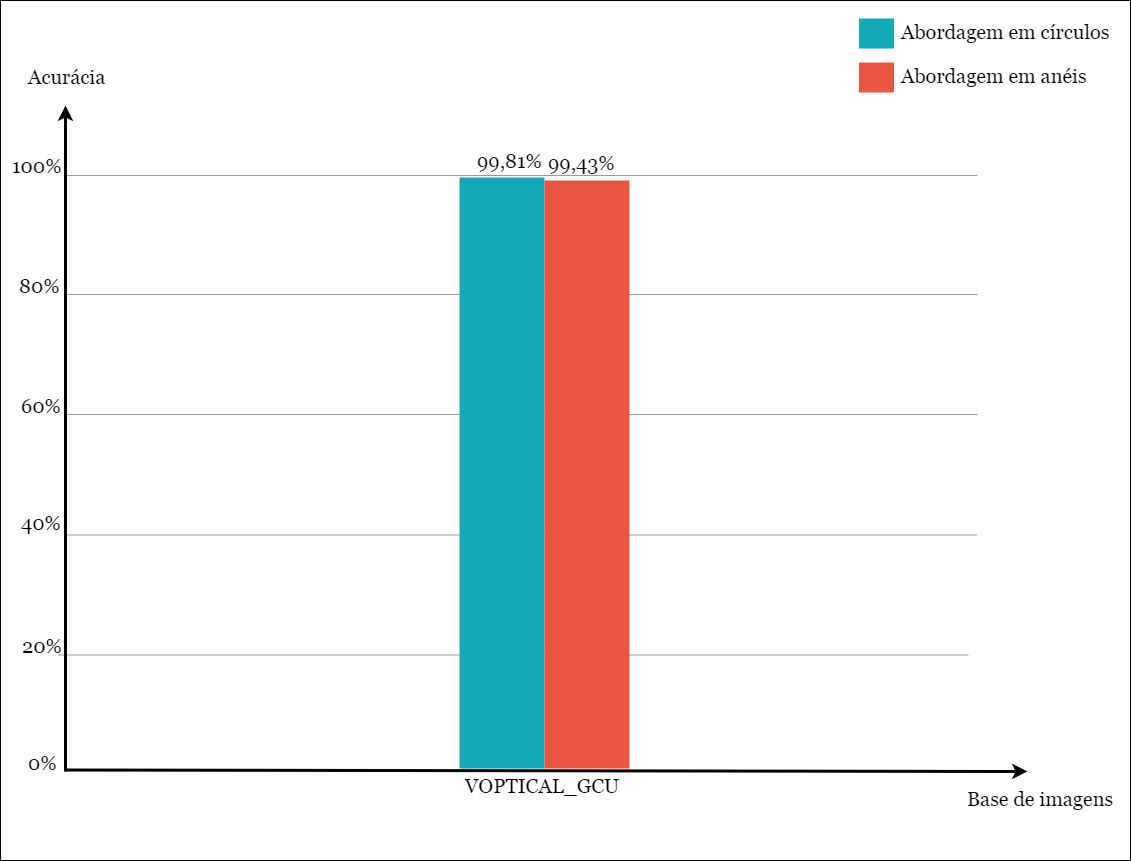
\includegraphics[width=0.8\textwidth]{figs/graficoKRipleyIndices.png}
    \legend{Fonte: Elaborado pela autora.}
    \label{fig:graficoIndicesDFKRipley}
\end{figure}

Finalizando, na Figura~\ref{fig:graficoIndicesDFKRipley} encontram-se os resultados da combinação dos índices de diversidade filogenética e a função K de \textit{Ripley} para a base de imagens capturada com o Interferômetro Doane (VOPTICAL\_GCU). Comparando os resultados produzidos para essa base de imagens, pode ser analisado que ao combinar os descritores, os resultados foram superiores aos produzidos usando somente a função K de \textit{Ripley} (Figura~\ref{fig:graficoKRipley}). Além disso, destaca-se que a abordagem em círculos produziu novamente o melhor resultado para a base VOPTICAL\_GCU, enfatizando que as informações cumulativas sobre as regiões do objeto, fornecidas pelo uso de círculos, são extremamente importantes para as imagens capturadas com o Interferômetro Doane. Entretanto, ambas abordagens apresentam bons resultados, concluindo que as características extraídas da função K de \textit{Ripley} e os índices de diversidade filogenética, possuem um alto poder de discriminação dos padrões de interferência da camada lipídica do filme lacrimal.

%Acreditamos, que o uso de anéis concêntricos elimina possíveis interferências de regiões centrais, fornecendo informações mais precisas a respeito das regiões periféricas da ROI..... Acreditamos que isso se deva às informações cumulativas sobre regiões periféricas do objeto, fornecidas pelo uso de círculos.

\section{Comparação do Método Proposto com os Trabalhos Relacionados}
\label{sec:comparacao}

Nesta seção é apresentada uma análise comparativa dos resultados obtidos pelo método proposto em relação aos trabalhos relacionados (Seção~\ref{sec:trabRelacionados}). A Tabela~\ref{tab:relacionados} apresenta um resumo desta comparação, fornecendo informações das técnicas, base de imagens, quantidade de imagens (amostra) e os valores médios de acurácia obtidos em cada trabalho.

Para realizar uma comparação mais rigorosa, os resultados obtidos em cada base do método proposto foi comparado com os trabalhos que utilizaram a mesma base de imagens, ou mesmo instrumento de captura das imagens. Entretanto, a comparação com outros trabalhos foi uma tarefa difícil, pois na literatura existem poucos trabalhos para quase todas as bases utilizadas no método proposto. Ainda assim, é possível elaborar alguns comentários em relação a esses trabalhos.

\definecolor{lightgray}{gray}{0.94}
\begin{table}[!ht]
\centering
\onehalfspacing
\caption{Comparação do método proposto com os trabalhos relacionados.}
\label{tab:relacionados}
\resizebox{\columnwidth}{!}{%
\begin{tabular}{lcp{8cm}cccc}
\cline{2-6} \parbox[t]{4mm}{\multirow{25}{*}{\rotatebox[origin=c]{90}{\textbf{Tearscope Plus}}}}
 & \textbf{Trabalho} & \centering \textbf{Técnica(s)} & \textbf{Base} & \textbf{Amostra} & \textbf{Acurácia} \\ \cline{2-6} 
 & (REMESEIRO et al., 2018) \cellcolor{lightgray} & Matriz de coocorrência no espaço de cor L*a*b* \cellcolor{lightgray} & VOPTICAL\_I1 \cellcolor{lightgray} & 105 \cellcolor{lightgray} & 96\% \cellcolor{lightgray}\\
 & (REMESEIRO et al., 2014) & Filtros \textit{Butterworth}, \textit{Gabor}, transformada discreta de \textit{Wavelet}, campos aleatórios de \textit{Markov} e coocorrência, seleção de características CFS, consistência e INTERACT & VOPTICAL\_I1 & 105 & 97,14\% \\
 & (MÉNDES et al., 2013) \cellcolor{lightgray} & Matriz de coocorrência, seleção de características CFS e método TOPSIS \cellcolor{lightgray} & VOPTICAL\_I1 \cellcolor{lightgray} & 105 \cellcolor{lightgray} & 95\% \cellcolor{lightgray}\\
 & (REMESEIRO et al., 2012) & Matriz de coocorrência em espaços de cores & VOPTICAL\_I1 & 105 & 96,19\% \\
 & (REMESEIRO et al., 2011) \cellcolor{lightgray} & Filtros \textit{Butterworth}, \textit{Gabor}, transformada discreta de \textit{Wavelet}, campos aleatórios de \textit{Markov} e coocorrência \cellcolor{lightgray} & VOPTICAL\_I1 \cellcolor{lightgray} & 105 \cellcolor{lightgray} & 96,19\% \cellcolor{lightgray}\\
 & (RAMOS et al., 2011) & Banco de filtros passa banda & VOPTICAL\_I1 & 105 & 91,43\% \\ \cline{2-6} 
 & (REMESEIRO et al., 2016) \cellcolor{lightgray} & Matriz de coocorrência, seleção de características CFS \cellcolor{lightgray} & VOPTICAL\_I1-v2 \cellcolor{lightgray} & 128 \cellcolor{lightgray} & 96,09\% \cellcolor{lightgray} \\ \cline{2-6} 
 & (REMESEIRO et al., 2014) & Filtros \textit{Butterworth}, \textit{Gabor}, transformada discreta de \textit{Wavelet}, campos aleatórios de \textit{Markov} e coocorrência, seleção de características CFS, consistência e INTERACT & VOPTICAL\_Is & 406 & 93,84\% \\ \cline{2-6} 
 & (CALVO et al., 2010) \cellcolor{lightgray} & Banco rotacionalmente invariante de filtros passa banda \cellcolor{lightgray} & PRIVADA \cellcolor{lightgray} & 91 \cellcolor{lightgray} & 86,41\% \cellcolor{lightgray}\\ \cline{2-6} \parbox[t]{5mm}{\multirow{4}{*}{\rotatebox[origin=c]{90}{\textbf{Int. Doane}}}}
 & (REMESEIRO et al., 2015) & Processamento de sinais, modelo e estatístico & VOPTICAL\_GCU & 106 & 93,40\% \\
 & (VILLAVERDE et al., 2014) \cellcolor{lightgray} & Processamento de sinais, modelo e estatístico e seleção de características CFS, consistência e INTERACT \cellcolor{lightgray} & VOPTICAL\_GCU \cellcolor{lightgray} & 106 \cellcolor{lightgray} & 91,51\% \cellcolor{lightgray}\\ \cline{2-6}
 & Método Proposto & Função K de \textit{Ripley} & \begin{tabular}[c]{@{}c@{}}VOPTICAL\_I1\\ VOPTICAL\_I1-v2\\ VOPTICAL\_ls\\ VOPTICAL\_GCU\end{tabular} & \begin{tabular}[c]{@{}c@{}}105\\ 128\\ 406\\ 106\end{tabular} & \begin{tabular}[c]{@{}c@{}}99,23\%\\ 93,12\%\\ 83,39\%\\ 95,28\%\end{tabular} \\ \cline{3-6} 
 &  & Índices de Diversidade Filogenética & VOPTICAL\_GCU & 106 & 97,36\% \\ \cline{3-6} 
 &  & Função K de \textit{Ripley} e Índices de Div. Filog. & VOPTICAL\_GCU & 106 & 99,81\% \\ \cline{2-6} 
\end{tabular}
}
\end{table}

\begin{comment}
\begin{table}[!ht]
\centering
\onehalfspacing
\caption{Comparação do método proposto com os trabalhos relacionados.}
\label{tab:relacionados}
\resizebox{\columnwidth}{!}{%
\begin{tabular}{cp{8cm}cccc}
\hline \hline
\textbf{Trabalho} & \textbf{Técnica(s)} & \textbf{Base} & \textbf{Amostra} & \textbf{Acurácia} \\ \hline \hline
\rowcolor{lightgray} (REMESEIRO et al., 2014) & Filtros \textit{Butterworth}, \textit{Gabor}, transformada discreta de \textit{Wavelet}, campos aleatórios de \textit{Markov} e coocorrência, seleção de características CFS, consistência e INTERACT & VOPTICAL\_I1 & 105 & 97,14\% \\
\rowcolor{lightgray} (REMESEIRO et al., 2012) & Matriz de coocorrência em espaços de cores & VOPTICAL\_I1 & 105 & 96,19\% \\
\rowcolor{lightgray} (REMESEIRO et al., 2011) & Filtros \textit{Butterworth}, \textit{Gabor}, transformada discreta de \textit{Wavelet}, campos aleatórios de \textit{Markov} e coocorrência & VOPTICAL\_I1 & 105 & 96,19\% \\
\rowcolor{lightgray} (REMESEIRO et al., 2018) & Matriz de coocorrência no espaço de cor L*a*b* & VOPTICAL\_I1 & 105 & 96\% \\
\rowcolor{lightgray} (MÉNDES et al., 2013) & Matriz de coocorrência, seleção de características CFS e método TOPSIS & VOPTICAL\_I1 & 105 & 95\% \\
\rowcolor{lightgray} (RAMOS et al., 2011) & Banco de filtros passa banda & VOPTICAL\_I1 & 105 & 91,43\% \\ \hline
(REMESEIRO et al., 2016) & Matriz de coocorrência, seleção de características CFS & VOPTICAL\_I1-v2 & 128 & 96,09\% \\ \hline
\rowcolor{lightgray} (REMESEIRO et al., 2014) & Filtros \textit{Butterworth}, \textit{Gabor}, transformada discreta de \textit{Wavelet}, campos aleatórios de \textit{Markov} e coocorrência, seleção de características CFS, consistência e INTERACT & VOPTICAL\_Is & 406 & 93,84\% \\ \hline
(CALVO et al., 2010) & Banco rotacionalmente invariante de filtros passa banda & PRIVADA & 91 & 86,41\% \\ \hline
\rowcolor{lightgray}(REMESEIRO et al., 2015) & Processamento de sinais, modelo e estatístico & VOPTICAL\_GCU & 106 & 93,40\% \\
\rowcolor{lightgray} (VILLAVERDE et al., 2014) & Processamento de sinais, modelo e estatístico e seleção de características CFS, consistência e INTERACT & VOPTICAL\_GCU & 106 & 91,51\% \\ \hline
Método Proposto & Função K de \textit{Ripley} & \begin{tabular}[c]{@{}c@{}}VOPTICAL\_I1\\ VOPTICAL\_I1-v2\\ VOPTICAL\_Is\\ VOPTICAL\_GCU\end{tabular} & \begin{tabular}[c]{@{}c@{}}105\\ 128\\ 406\\ 106\end{tabular} & \begin{tabular}[c]{@{}c@{}}99,23\%\\ 93,12\%\\ 83,39\%\\ 95,28\%\end{tabular} \\ \cline{2-5} 
 & Índices de Diversidade Filogenética & VOPTICAL\_GCU & 106 & 97,36\% \\ \cline{2-5} 
 & Função K de \textit{Ripley} e Índices de Div. Filog. & VOPTICAL\_GCU & 106 & 99,81\% \\ \hline
\end{tabular}
}
\end{table}
\end{comment}

No trabalho de \citeonline{calvo2010color} a base privada utilizada é composta por imagens capturadas com o Teascope Plus, portanto é possível realizar comparação com as bases de imagens VOPTICAL\_I1, VOPTICAL\_I1-v2 e VOPTICAL\_Is utilizadas no método proposto, pois são capturadas com o mesmo instrumento. Em relação aos trabalhos que usaram a base de imagens VOPTICAL\_I1, é possível observar que a performance do método proposto que usa a mesma base foi superior a todos os trabalhos, em termos de acurácia.

%Os trabalhos que usaram as bases de imagens VOPTICAL\_I1-v2 e VOPTICAL\_Is, obtiveram taxas de acerto maiores que as do método proposto. Entretanto, a quantidade de amostras das bases VOPTICAL\_I1-v2 e VOPTICAL\_Is usadas no método proposto, são expressivamente maiores do que as utilizadas no trabalho de \citeonline{calvo2010color}, sendo 28,91\% e 77,59\% superiores. Um número maior de amostras aumenta a heterogeneidade e, consequentemente leva os experimentos a estarem sob circunstâncias mais realistas.

Os trabalhos que usaram as bases de imagens VOPTICAL\_I1-v2 e VOPTICAL\_Is obtiveram taxas de acerto maiores que as do método proposto, porém próximos. Em relação a base privada, é possível observar que o resultado alcançado é inferior aos resultados produzidos pelo método proposto, e a quantidade de amostras das bases VOPTICAL\_I1-v2 e VOPTICAL\_Is são expressivamente maiores do que as utilizadas na base privada, sendo superior 28,91\% e 77,59\%, respectivamente. É importante destacar que um número maior de amostras aumenta a heterogeneidade e, consequentemente leva os experimentos a estarem sob circunstâncias mais realistas.

Os trabalhos de \citeonline{remeseiro2015automatic} e \citeonline{villaverde2014feature} realizam testes na base de imagens VOPTICAL\_GCU. Observando os resultados desses trabalhos e comparando com os resultados alcançados no método proposto quando usa a base VOPTICAL\_GCU, é possível verificar que o método proposto apresenta resultados superiores aos dois trabalhos, tanto ao aplicar somente o descritor da função K de \textit{Ripley} ou os índices de diversidade filogenética, quanto concatenando ambos descritores. 

Finalmente, é importante destacar que neste trabalho é realizada uma análise detalhada dos resultados, por meio das médias obtidas na acurácia, desvio padrão, área sob a curva ROC, \textit{Kappa} e \textit{F-Measure}, isto é, não são considerados apenas resultados isolados. Dessa forma, é possível verificar a consistência dos resultados produzidos para discriminação dos padrões.

Vale ressaltar que o objetivo deste trabalho não é superar todas as metodologias descritas na literatura, mas contribuir com o desenvolvimento de um novo método automático para classificar os padrões de interferência da camada lipídica em imagens do filme lacrimal.

\section{Considerações Finais}

Neste capítulo foram apresentados e discutidos os resultados obtidos pelos experimentos realizados no desenvolvimento do método proposto. Também foi feito um comparativo com os trabalhos relacionados, como forma de analisar a relevância da pesquisa desenvolvida.

No geral, os resultados obtidos podem ser considerados promissores, sendo
comparáveis aos melhores trabalhos descritos na literatura. As maiores taxas de acerto
foram obtidas com a utilização do algoritmo \textit{Greedy Stepwise} para seleção das características mais relevantes da junção dos descritores da função K de \textit{Ripley} e índices de diversidade filogenética, onde foi possível alcançar valores médios de acurácia superiores a 99\%.

No próximo capítulo são apresentadas as conclusões a cerca da pesquisa desenvolvida nesta dissertação. Também serão apontadas algumas de suas limitações, bem como apresentadas sugestões para trabalhos futuros.